\documentclass{standalone}
\usepackage{pgfplots}
\usetikzlibrary{shapes.geometric, intersections}
\pgfplotsset{compat=1.7}

\begin{document}
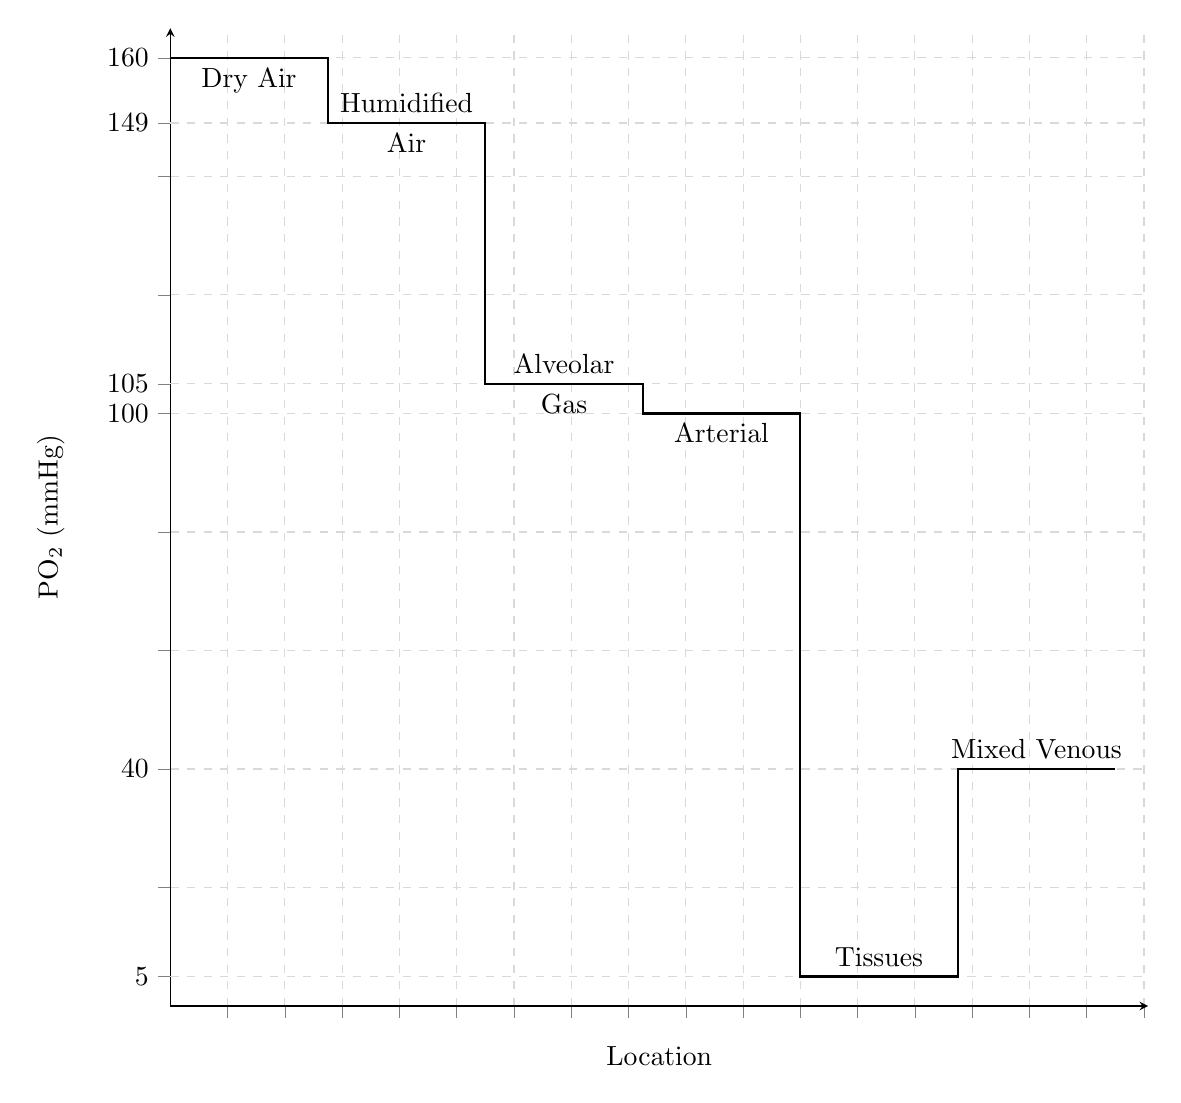
\begin{tikzpicture}

    \begin{axis}[
        axis x line=middle,
        axis y line=middle,
        x tick label style={/pgf/number format/fixed,
                            /pgf/number format/fixed zerofill,
                            /pgf/number format/precision=1},
        y tick label style={/pgf/number format/fixed,
                            /pgf/number format/fixed zerofill,
                            /pgf/number format/precision=0},
        grid = major,
        width=14cm,
        height=14cm,
        grid style={dashed, gray!30},
        xmin=0,     % start the diagram at this x-coordinate
        xmax= 12cm,    % end   the diagram at this x-coordinate
        ymin= 0,     % start the diagram at this y-coordinate
        ymax= 165,   % end   the diagram at this y-coordinate
        %axis background/.style={fill=white},
    	  x label style={at={(axis description cs:0.5,-0.1)},anchor=north},
	  y label style={at={(axis description cs:-0.1,.5)},rotate=90,anchor=south},
	  xticklabels={},
	 yticklabels={,,,40,,,100,,,160},
	extra y ticks={5,105,149},
	extra y tick labels = {5,105,149},
	 ylabel near ticks,
	xlabel near ticks,
        xlabel=Location,
        ylabel=PO\textsubscript{2} (mmHg),
        tick align=outside,
        enlargelimits=false]

	\draw [thick, black] (0cm,160)-- node[below] {Dry Air} (2cm,160)--(2cm,149)--node[below] {Air} node[above] {Humidified} (4cm,149)--(4cm,105)--node[below] {Gas} node[above] {Alveolar}(6cm,105)--(6cm,100)--node[below] {Arterial}(8cm,100)--(8cm,5)--node[above] {Tissues}(10cm,5)--(10cm,40)--node[above] {Mixed Venous}(12cm,40);

\end{axis}

\end{tikzpicture} 
\end{document}